\documentclass[a4paper,11pt]{report}

% -- Typography --
\usepackage[utf8]{inputenc}
\usepackage[%
    tracking=true,%
    kerning=true,%
    selected=true,%
    stretch=15,%
    shrink=15,%
]{microtype}

% -- Math --
\usepackage{amsmath}
\usepackage{amsfonts}
\usepackage{amsthm}

\theoremstyle{plain}
\newtheorem{thm}{Theorem}[section]
\newtheorem{lem}[thm]{Lemma}

\theoremstyle{definition}
\newtheorem{defn}[thm]{Definition}

% -- Tables --
\usepackage{booktabs}

% -- Graphics --
\usepackage{pgfplots}

% -- TOC --
\usepackage[nottoc,section]{tocbibind}
\usepackage[titles]{tocloft}

% -- Misc. --
\usepackage[plain]{fancyref}
\usepackage{hyperref}
\usepackage{color}
\usepackage{array}
\usepackage{url}

\usepackage{tikz}
\usetikzlibrary{arrows,petri,topaths}
\usepackage{tkz-berge}

\usepackage[labelfont=bf]{caption}
\usepackage{subcaption}

% -- Bookkeeping --
\setcounter{secnumdepth}{3}
\renewcommand{\thesection}{\arabic{section}}
\settocbibname{References}

\begin{document}

% -- Title --
\title{Proving the Correctness of Prim's Algorithm for Computing
Minimum Spanning Trees}
\author{Siddharth Mahendraker\\
    \url{siddharth.mahen@gmail.com}}
\maketitle

% -- TOC --
\renewcommand{\cfttoctitlefont}{\Large\bfseries}
\setlength\cftaftertoctitleskip{1em}
\setlength\cftbeforesecskip{0.5em}

\setcounter{page}{1}
\pagenumbering{roman}
\tableofcontents
\clearpage
\setcounter{page}{1}
\pagenumbering{arabic}

\section{Motivation}

% We motivate the study of MSTs and the correctness of Prim's algorithm using
% the following example.

Consider the following scenario. A group of 11th grade IB students are big
basketball fans. Today, their favourite team is playing their arch rivals.
The students watch the game during lunch, but unfortunately, the end of the
game overlaps with their next class.

Itching to know how the game ends, the students decide to designate one
student as a broadcaster, who will discretely read the game's twitter
feed from his phone and tell everyone else what's going on. The students
decide this broadcaster will tell his neighbours the news, and they will in
turn tell their neighbours and so forth, until everyone in the class has
been updated. The students agree this method will arouse the least amount
of suspicion from their strict teacher, who already separates their desks
to keep talking to a minimum.

At first, their strategy works well, however, they notice that some of their
methods of passing messages are less risky than others. Particularly, they
notice that it is sometimes less risky for a student to update only a few of
his neighbours directly, and let the information reach his other neighbours
indirectly via other people.

Interested in repeating this strategy for other basketball games in other
classes, the students ask themselves: How can we pass messages around
the classroom such that our total risk is minimized, but everyone receives
updates about the game?

\section{Minimum Spanning Trees}

The students' dilemma can be modelled using graph theory. Let $G = (V, E, w)$
be a simple, connected, weighted graph whose vertices correspond to students
and whose edges correspond to opportunities to pass messages, where the weight
$w(e)$ of an edge $e \in E$ corresponds to the risk that the conversation
between the students $u,v$ at the ends of $e$ is compromised (see
\Fref{fig:class-graph}). Call $G$ the students' classroom graph.

\begin{figure}[t]
  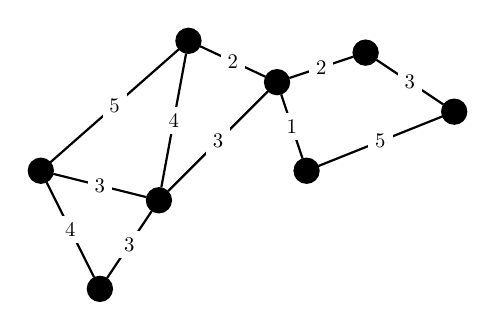
\begin{tikzpicture}[scale=0.75,transform shape]
  \SetVertexMath
  \GraphInit[vstyle=Simple]
  \SetGraphUnit{2.5}
  \Vertex[x=0,y=2]{A}
  \Vertex[x=1,y=0]{B}
  \Vertex[x=2,y=1.5]{C}
  \Vertex[x=2.5,y=4.2]{D}
  \Vertex[x=4,y=3.5]{E}
  \Vertex[x=4.5,y=2]{F}
  \Vertex[x=5.5,y=4]{G}
  \Vertex[x=7,y=3]{H}
  \Edge[label=$5$](A)(D)
  \Edge[label=$4$](A)(B)
  \Edge[label=$3$](A)(C)
  \Edge[label=$4$](D)(C)
  \Edge[label=$3$](C)(B)
  \Edge[label=$2$](D)(E)
  \Edge[label=$3$](C)(E)
  \Edge[label=$1$](E)(F)
  \Edge[label=$2$](E)(G)
  \Edge[label=$3$](G)(H)
  \Edge[label=$5$](F)(H)
\end{tikzpicture}
\centering
\caption{A graph representing a possible arrangement of students in the
classroom. Vertices represent students and edges represent opportunities to
pass messages, where the weight of an edge represents the risk that the
conversation across the edge is compromised.}
\label{fig:class-graph}
\end{figure}


For the remainder of this paper, all graphs are assumed to be simple and
undirected, and all weights are assumed to be positive. Recall that a graph is
connected if there exists a path between every vertex $u$ and $v$ in the graph.

\begin{defn}
Let $G$ be a graph. We call $G$ \emph{connected} if there is
a sequence of adjacent edges, i.e.~a path,  between every vertex $u$ and $v$
in $G$.
\end{defn}

An ideal method of passing messages would require that the students find
a set of opportunities to pass messages, $E' \subset E$, such that the total
risk the students run is as low as possible, and every student receives
updates about the game. This corresponds to some subgraph $T = (V, E', w)$
of the classroom graph $G$.

%% Avoid using words like immediately; condescending to the reader

Immediately, we see that any cyclic subgraph $T$ of the classroom graph can
never be considered a low risk method of passing messages. This is a
consequence of trying to minimize the total risk the students run. Suppose the
students come up with some connected cyclic subgraph $T = (V, E', w)$ which
they want to use to pass messages. We can create a new subgraph $T^*$ of $T$ by
removing an edge from each of the cycles in $T$. This new subgraph has a lower
risk of getting the students caught as it contains strictly fewer edges than
$T$.  Moreover, because removing single edges from cycles preserves the
connectedness in $T$, this subgraph can still be used to pass messages to
everyone. Therefore, since we can always construct a lower risk subgraph given
a cyclic subgraph, we won't bother considering cyclic subgraphs to pass
messages.

\begin{defn}
Let $G = (V, E)$ be a connected graph. Then a \emph{spanning tree} $T$ of $G$
is defined as a connected acyclic subgraph $T = (V, E')$, where $E' \subset
E$.
\end{defn}

Reformulating the students' problem, we say the students are looking for a
spanning tree $T$ of the classroom graph $G$ where the sum of the weights of
the edges in the spanning tree are as low as possible (or at least as low as
that of any other spanning tree of $G$).

\begin{defn}
Let $T = (V, E', w)$ be a spanning tree of a weighted graph $G = (V, E, w)$.
Define the cost of the spanning tree, $c(T)$ as the sum of the edge weights in
$E'$,
\begin{equation*}
    c(T) = \sum_{e \in E'}{w(e)}.
\end{equation*}
\end{defn}

If a spanning tree $T$ of a graph $G$ has a cost at least as low as the
cost of every other possible spanning tree of $G$, we call $T$ a minimum
spanning tree of $G$.

\begin{defn} Let $T^*$ be a spanning tree of a graph $G$. We call $T^*$ a
\emph{minimum spanning tree} (MST) if
\begin{equation*}
    c(T^*) \leq c(T)
\end{equation*}
for all alternate spanning trees $T$ of $G$.
\end{defn}

Given a minimum spanning tree, it is evident the students could achieve their
goal of communicating updates to everyone while minimizing the total risk they
run. The broadcaster would simply send his messages to students adjacent to
him in the minimum spanning tree, and these students would simply propagate
their messages to their neighbours on the spanning tree and so forth. Because
the minimum spanning tree represents a way of propagating messages with the
lowest total risk, and every student is part of the minimum spanning tree, it
constitutes an optimal solution.

However, there still remains the problem of actually computing a minimum
spanning tree for the classroom graph. Assuming the students have an accurate
idea of the risk involved in speaking with any of their neighbours, how can the
students compute a minimum spanning tree for their classroom graph?
Furthermore, how can they be sure the spanning tree they compute is truly a
\emph{minimum} spanning tree?

%% say something like: the remainder of this paper is devoted to proving..
%% better transitions between topics

\section{Prim's Algorithm for Computing MSTs}

The following algorithm, due to Robert C. Prim, can be used to compute
the minimum spanning tree $T^*$ of a weighted graph $G$
\cite[pp. 634--636]{clrs}.

\begin{defn}[{\bfseries Prim's Algorithm}] Let $G = (V, E, w)$ be a
weighted graph. Then a minimum spanning tree $T^*$ of $G$ can be computed as
follows:
\begin{enumerate}
    \item Begin with an empty set $T = \emptyset$ and a set $X
    = \left\{v\right\}$, where $v \in V$ is arbitrarily selected.
    \item Until $X = V$ repeat the step below.
    \item Let $Y$ be the set edges with one vertex in $X$ and the other
    vertex in $E - X$. Choose the edge $e \in Y$ with the smallest weight
    $w(e)$, breaking ties arbitrarily. Add $e$ to $T$ and add the vertex at
    the other end of $e$ to $X$.
    \item Output a minimum spanning tree $T^* = (V, T, w)$.
\end{enumerate}
\end{defn}

See \Fref{fig:prim-example} for an example of how Prim's algorithm works.

Intuitively, this algorithm corresponds to the following strategy for the
students:

\begin{enumerate}
    \item Begin with an arbitrarily selected broadcaster.
    \item Have the broadcaster pick a neighbour who, when spoken to, is least
    likely to compromise the pair. Pass messages to this neighbour.
    \item Now, with respect to the current group of people who know the news,
    pick a neighbour who, when spoken to, is least likely to compromise the
    group.
    \item Repeat the previous step until everyone in the class knows the latest
    information.
\end{enumerate}

\begin{figure}[t]
\centering
\begin{subfigure}[t]{0.4\textwidth}
\centering
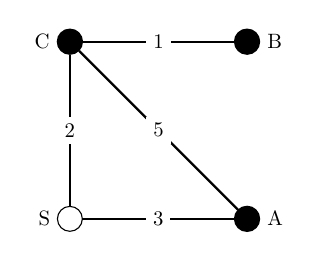
\begin{tikzpicture}[scale=0.75,transform shape]
\GraphInit[vstyle=Classic]
\SetGraphUnit{2.5}
\Vertex[x=3,y=0]{A}
\Vertex[x=3,y=3]{B}
\Vertex[x=0,y=3,Lpos=180]{C}
\tikzset{VertexStyle/.style = {
shape = circle,
fill = white,
inner sep = 0pt,
outer sep = 0pt,
minimum size = 12pt,
draw}}
\Vertex[x=0,y=0,Lpos=180]{S}
\Edge[label=$2$](S)(C)
\Edge[label=$3$](S)(A)
\Edge[label=$1$](C)(B)
\Edge[label=$5$](C)(A)
\end{tikzpicture}
\caption{}
\end{subfigure}
\;
\begin{subfigure}[t]{0.4\textwidth}
\centering
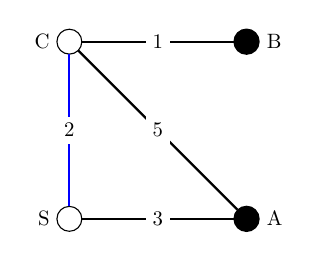
\begin{tikzpicture}[scale=0.75,transform shape]
\GraphInit[vstyle=Classic]
\SetGraphUnit{2.5}
\Vertex[x=3,y=0]{A}
\Vertex[x=3,y=3]{B}
\tikzset{VertexStyle/.style = {
shape = circle,
fill = white,
inner sep = 0pt,
outer sep = 0pt,
minimum size = 12pt,
draw}}
\Vertex[x=0,y=0,Lpos=180]{S}
\Vertex[x=0,y=3,Lpos=180]{C}
\Edge[local,label=$2$,color=blue](S)(C)
\Edge[label=$3$](S)(A)
\Edge[label=$1$](C)(B)
\Edge[label=$5$](C)(A)
\end{tikzpicture}
\caption{}
\end{subfigure}

\vspace{10pt}
\begin{subfigure}[t]{0.4\textwidth}
\centering
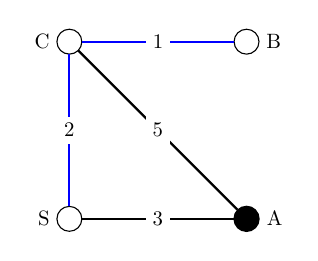
\begin{tikzpicture}[scale=0.75,transform shape]
\GraphInit[vstyle=Classic]
\SetGraphUnit{2.5}
\Vertex[x=3,y=0]{A}
\tikzset{VertexStyle/.style = {
shape = circle,
fill = white,
inner sep = 0pt,
outer sep = 0pt,
minimum size = 12pt,
draw}}
\Vertex[x=0,y=0,Lpos=180]{S}
\Vertex[x=0,y=3,Lpos=180]{C}
\Vertex[x=3,y=3]{B}
\Edge[local,label=$2$,color=blue](S)(C)
\Edge[local,label=$1$,color=blue](C)(B)
\Edge[label=$3$](S)(A)
\Edge[label=$5$](C)(A)
\end{tikzpicture}
\caption{}
\end{subfigure}
\;
\begin{subfigure}[t]{0.4\textwidth}
\centering
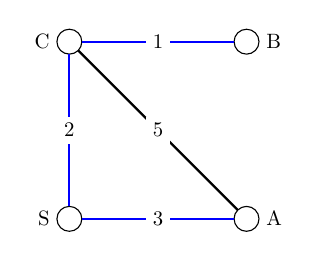
\begin{tikzpicture}[scale=0.75,transform shape]
\GraphInit[vstyle=Classic]
\SetGraphUnit{2.5}
\tikzset{VertexStyle/.style = {
shape = circle,
fill = white,
inner sep = 0pt,
outer sep = 0pt,
minimum size = 12pt,
draw}}
\Vertex[x=0,y=0,Lpos=180]{S}
\Vertex[x=0,y=3,Lpos=180]{C}
\Vertex[x=3,y=3]{B}
\Vertex[x=3,y=0]{A}
\Edge[local,label=$2$,color=blue](S)(C)
\Edge[local,label=$1$,color=blue](C)(B)
\Edge[local,label=$3$,color=blue](S)(A)
\Edge[label=$5$](C)(A)
\end{tikzpicture}
\caption{}
\end{subfigure}
\caption{The execution of Prim's algorithm on a weighted graph $G$ with 4
vertices. White vertices represent elements of $X$, while black vertices
represent elements of $V - X$. Blue edges represent edges added to the
output spanning tree $T^*$. In step (a), the inital element $S \in X$ is
chosen arbitrarily. We see that in step (d), Prim's algorithm halts as $X = V$
and $T^*$ is indeed a minimum spanning tree of $G$.}
\label{fig:prim-example}
\end{figure}



Apart from their utility in colluding against teachers, minimum spanning trees
have a myriad of other important applications. They provide a solution to a
vast array of real world optimization problems, in fields as disparate as
computer networking, machine learning and infrastructure construction. From the
fairly trivial scenario used above, we see that computing a minimum spanning
trees is an important part of broadcasting information efficiently among a set
of interconnected parties. Therefore, it is important to know whether
algorithms such as Prim's algorithm really do work correctly to output minimum
spanning trees.

My personal interest in analyzing minimum spanning tree algorithms grew out of
my interest in their asymptotic running time analyses. Particularly, the
analysis of a randomized algorithm to compute minimum spanning trees very
efficiently for arbitrary graphs, due to Karger, Klein and Tarjan. For more
information see \cite{linear-rand-mst}.

The remainder of this paper is devoted to proving the correctness of
Prim's algorithm.

The proof of correctness will proceed in three parts. First, we show that the
algorithm terminates. Then we show that it outputs a spanning tree. Finally,
we show that the output spanning tree is minimal.

\section{Connectedness and the Cut Lemma}

Before we begin, let us establish an important property of connected graphs,
which will allow us to more easily navigate the proofs ahead.

The motivation behind the following lemma is that it allows us to clearly link
what Prim's algorithm does in every step to the connectedness of its
input graph. In every step, the algorithm adds an edge $e$ to $T$ with one
endpoint in $X$ and another endpoint in $V - X$. If we can show that for any
choice of $X$ and $V - X$, this edge $e$ always exists, then we can easily
deduce many other properties of the algorithm.

\begin{lem}[{\bfseries The Cut Property}]
Let $G = (V, E, w)$ be a weighted graph. Then $G$ is connected
if and only if for any partition of $V$ into two sets $A$, $B$ such that
$A \cup B = V$ and $A \cap B = \emptyset$, there exists at least
one edge with a vertex in $A$ and a vertex in $B$, i.e., an edge which
crosses the cut $(A, B)$.

\begin{proof}
Assume $G$ is connected. Then there exists a path between every vertex $u$ and
$v$ in $V$. Let $A$ and $B$ be an arbitrary partition of $V$ such that
$A \cup B = V$ and $A \cap B = \emptyset$. Now suppose $a \in A$ and $b \in B$
are two vertices on different sides of the partition. Then by the connectedness
of $G$, there exists a sequence of edges between $a$ and $b$. Because $a$ and
$b$ are on different sides of the partition, there must be some edge $e \in E$
which has one endpoint in $A$ and the other endpoint in $B$. Hence, there
exists a cut which crosses $(A, B)$. Since $A$ and $B$ were chosen arbitrarily,
we've shown connectedness implies the cut property.

Now, assume that for all partitions $A$, $B$ of a graph $G$, and there
exists at least one edge $e \in E$ which has a vertex in $A$ and a vertex in
$B$. First, we show that for any choice of $A$ and $B$, $A$ and $B$ are
connected.

Suppose $A$ is not connected. Then there exist vertices $x_1, x_2, \ldots, x_k$
in $A$ which cannot be connected by a path. Let $X \subset A$ denote the
set of vertices which can be reached from $x_1$ by a path. Assume, without loss
of generality, that $B$ is connected, and the edge across $(A, B)$ has an
endpoint in $X$. Then for the partition $X \cup B$ and $A - (X \cup B)$ there
do not exist any edges which cross the cut $(X \cup B, A - (X \cup B))$, a
contradiction. Hence, $A$ must be connected. Similarly, $B$ must be connected.

Since $A$ and $B$ are connected by the edge $e$ and $A \cup B = V$, the entire
graph $G$ is connected. Therefore, we've shown the cut property implies
connectedness.
\end{proof}
\end{lem}

\section{Proof of Correctness of Prim's Algorithm}

Using the cut property, proving the correctness of Prim's algorithm becomes
much simpler.

Recall that proving the correctness of Prim's algorithm requires proving the
algorithm terminates, that it outputs a spanning tree of the input graph, and
that this spanning tree is minimal.

\begin{thm}
Let $G = (V, E, w)$ be a connected, weighted graph. Then the
execution of Prim's algorithm for the input $G$ eventually terminates.

\begin{proof}
In each step of Prim's algorithm, an edge $e$ is added to $T$, with one
endpoint $u \in X$ and another endpoint $v \in V - X$. The endpoint $v$ is then
added to $X$. By the cut property, we know that such an edge exists for all
cuts across $(X, V - X)$. Therefore, after every step of the algorithm, an
endpoint $v \in V - X$ of an edge $e$ is added to $X$, and hence the
cardinality of $X$ increases by $1$. Since the cardinality of $X$ begins at
$1$, and the cardinality of $V$ is finite, there must exist some step after
which $X = V$. Hence, Prim's algorithm must terminate.
\end{proof}
\end{thm}

\begin{thm}
Let $G = (V, E, w)$ be a connected, weighted graph. Then the output
$T^* = (V, T, w)$ of the execution of Prim's algorithm for the input $G$
constitutes a spanning tree of $G$.

\begin{proof}
First, we show that the output of Prim's algorithm $T^*$ is always connected,
using induction on the number of steps of the algorithm.

In the base case, let $X = \left\{v\right\}$. Then by the cut property, we
know there exists an edge $e \in E$ across the cut $(X, V - X)$. Adding the
endpoint of $v'$ of $e$ to $X$ and the edge $e$ to $T$ clearly leaves $T^*$
connected as there is a path between all the vertices in $T^*$.

Now assume $T^*$ is connected at after some step $k$. We show that $T^*$ is
still connected after step $k + 1$. By the cut property, we know that in any
step of the algorithm, there exists an edge $e$ across the cut $(X, V - X)$,
where the endpoint of the cut $v' \in V - X$ is not in $T^*$. Hence, assuming
$T^*$ is connected, adding the vertex $v'$ to $X$ and the edge $e$ to $T$
leaves $T^*$ connected at the end of step $k + 1$. Therefore, by induction,
$T^*$ is always connected.

Next, we show that $T^*$ never contains any cycles. In any step of the
algorithm, the only way to create a cycle is to add an edge $e$ to $T$
with both endpoints $x$ and $x'$ in $X$ when there already exists a path
between $x$ and $x'$. By definition, however, the algorithm only adds edges
to $T$ with one endpoint in $X$ and the other in $V - X$. Therefore,
$T^* = (X, T, w)$ must be acylic after every step of the algorithm.

Since Prim's algorithm terminates when $X = V$, and the output
$T^* = (X, T, w)$ is always connected and acyclic, the output of Prim's
algorithm constitutes a spanning tree of the original graph $G$.
\end{proof}
\end{thm}

\begin{thm}
Let $G = (V, E, w)$ be a connected, weighted graph. Then the output
$T^* = (V, T, w)$ of the execution of Prim's algorithm for the input $G$
constitutes a minimum spanning tree of $G$.

\begin{proof}
Let $S^* = (V, S, w)$ be a minimum spanning tree of $G$. From the previous
theorem, we know that $T^*$ is a spanning tree of $G$. We show that the weight
of every edge in $T^*$ is at least as small as the weight of every edge in
$S^*$, and thus that $T^*$ is also a minimum spanning tree of $G$.

Consider the execution of Prim's algorithm in some step $k$. Let $e_k$ be the
edge across the cut $(X, V - X)$ which was added to $T$, and let $e^* \in S$ be
the edge across $(X, V - X)$ in $S^*$. We know $S^*$ must have an edge across
the cut $(X, V - X)$ as $S^*$ is connected. Now consider the weights of the
edges $e_k$ and $e^*$. By definition, Prim's algorithm chooses an edge across
the cut $(X, V - X)$ with the lowest weight, and thus $w(e_k) \leq w(e^*)$.
Since this holds in any arbitrary step $k$, we conclude that
\begin{align*}
    \sum_{e \in T}{w(e)} = c(T^*) \leq c(S^*) = \sum_{e \in S}{w(e)}.
\end{align*}
If $c(T^*) < c(S^*)$, then $S^*$ is not a minimum spanning tree, a
contradiction. Thus $c(T^*) = c(S^*)$.  Therefore, the output of Prim's
algorithm, $T^*$, constitutes a minimum spanning tree of the input graph $G$.
\end{proof}
\end{thm}

Note that no step in the three precedent proofs was dependent on the choice of
the initial vertex $S \in X$, and thus this element can be selected arbitrarily
without consequence.

\section{Conclusion}

We conclude that Prim's algorithm is indeed correct; given a connected weighted
graph $G$ as input, it outputs a truly \emph{minimum} spanning tree of $G$.
Great! This means the students can always compute a lowest risk method of
passing messages to one another in their classroom graph (see
\Fref{fig:class-graph-mst}).

\begin{figure}[t]
  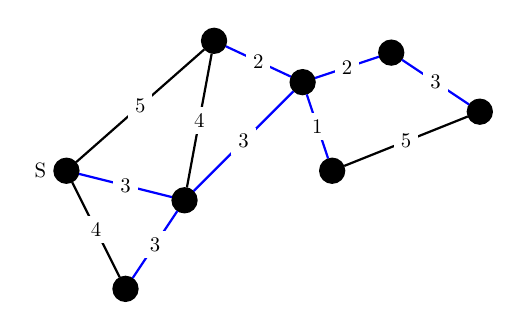
\begin{tikzpicture}[scale=0.75,transform shape]
  \SetVertexMath
  \GraphInit[vstyle=Simple]
  \SetGraphUnit{2.5}
  \Vertex[x=0,y=2,L=$S$,NoLabel=false,LabelOut=true,Lpos=180]{A}
  \Vertex[x=1,y=0]{B}
  \Vertex[x=2,y=1.5]{C}
  \Vertex[x=2.5,y=4.2]{D}
  \Vertex[x=4,y=3.5]{E}
  \Vertex[x=4.5,y=2]{F}
  \Vertex[x=5.5,y=4]{G}
  \Vertex[x=7,y=3]{H}
  \Edge[label=$5$](A)(D)
  \Edge[label=$4$](A)(B)
  \Edge[label=$4$](D)(C)
  \Edge[label=$5$](F)(H)
  \Edge[local,label=$3$,color=blue](A)(C)
  \Edge[local,label=$3$,color=blue](C)(B)
  \Edge[local,label=$2$,color=blue](D)(E)
  \Edge[local,label=$3$,color=blue](C)(E)
  \Edge[local,label=$1$,color=blue](E)(F)
  \Edge[local,label=$2$,color=blue](E)(G)
  \Edge[local,label=$3$,color=blue](G)(H)
\end{tikzpicture}
\centering
\caption{The output of Prim's algorithm given the example classroom graph from
\Fref{fig:class-graph} as input. Blue edges represent edges in the output
spanning tree. The initial vertex $S$ was chosen arbitrarily. It is not
difficult to see that the output spanning tree would be the same had the
algorithm selected any other initial vertex.}
\label{fig:class-graph-mst}
\end{figure}


Although we have shown that Prim's algorithm is correct, there are many other
aspects of minimum spanning tree computation that are still of interest. For
example, if we change the weights of $m$ edges in the input graph, how could we
recompute an MST of the input graph efficiently? This question comes up very
often when MSTs are used in relation to communication networks, where the
strengths of communications channels can vary over time. See
\cite[§8]{eisner97} for a complex yet thorough solution to this problem.

Moving further away from practical applications of MST computation, we could
also ask whether MSTs and algorithms such as Prim's algorithm provide good
approximate solutions to other problems. For example, consider using MST
computation to approximate solutions to the Travelling Salesman Problem. We
could also ask whether Prim's algorithm could be modified to handle negative
edge weights.

\bibliographystyle{plain}
\bibliography{doc.bib}

\end{document}
